% Chapter 1

\chapter{Introduction} % Main chapter title

\label{Chapter1} % For referencing the chapter elsewhere, use \ref{Chapter1} 

%----------------------------------------------------------------------------------------

% Define some commands to keep the formatting separated from the content 
\newcommand{\keyword}[1]{\textbf{#1}}
\newcommand{\tabhead}[1]{\textbf{#1}}
\newcommand{\code}[1]{\texttt{#1}}
\newcommand{\file}[1]{\texttt{\bfseries#1}}
\newcommand{\option}[1]{\texttt{\itshape#1}}

%----------------------------------------------------------------------------------------

\section{Introduction of Contact problems}
The contact problems are very importance in industrial applications in mechanical and civil engineering. The range of application are profusely such as metal forming processes, drilling problems, bearings or crash analysis of cars. Other applications are related to biomechanics where human joints, implant or teeth are considered. Due to this variety contact problems are today combined either with large elastic or inelastic deformations
including time dependent responses. Thermal coupling might have to be considered, see the cooling of electronic devices, the heat removal within nuclear power plant vessels or
thermal insulation of astronautic vehicles. Even stability behavior has to be linked tocontact, like wrinkling arising in metal forming problems. \parencite{ref1} Due to this technical importance a great number of researchers have investigated contact
problems. Starting with the classical analytical work of Hertz (1882) on the elastic contact of two spheres the deformation of the bodies being in contact has been taken into account. However only very few problems involving contact can be solved analytically. Thus for
most industrial applications numerical methods have to be applied when the contacting bodies have complex geometries . Due to that the solution of contact problems with finite
element methods has a relatively long history. \parencite{ref1}
The following introductory remarks are related to the steps which have to be followed when
treating contact problems within the finite element method. \parencite{ref1}


%----------------------------------------------------------------------------------------

\section{ Introduction of Hyper-elastic materials}
Hyper-elastic materials are designed for modeling rubber or rubber-like materials in which the elastic deformation can be extremely large. 

\begin{figure}[H]
    \centering
    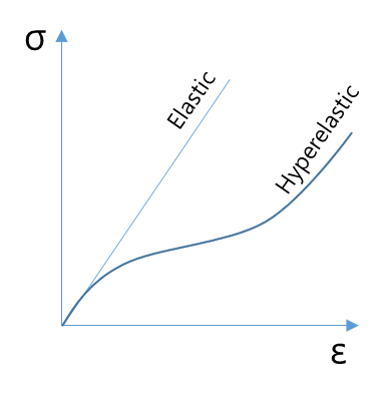
\includegraphics[scale=1]{Figures/Hyperelastic.png}
    \decoRule   
    \caption{ Introduction of hyper-elastic materials.}
    \label{fig:Electron}
\end{figure}
Hyper-elastic materials use something called a strain energy density function to derive the relationship between stress and strain. This allows them to model the relationship between stress and strain accurately even when the strain is between 100 \% to 700 \%, depending on the exact hyper-elastic model that is used.
Various hyper-elastic models are accurate over different range of strains. You must choose the model to use depending on the expected range of strains, the computational expense of the formulation and the amount of data that you have to define in the stress-strain relationship.

\section{Study objective}
In this study, contact problems with hyper-elastic materials will be considered in cases of frictionless sliding and frictionless compressing and the obtained results will be verified with the solution given by commercial program. From the theories and algorithms about contact problems and hyper – elastics materials based on finite element method, some
programs have to be made to resolve the problem of contact for hyper – elastic materials. These example will be programmed by using MATLAB and Python programming
languages, then the results which will be obtained from these programs will be compared to the results of commercial program (ANSYS).


